\chapter{評価}
\label{chap:evaluation}
\section{1人麻雀による和了率の比較}
提案手法で提示した、期待和了順目の評価による打牌選択のアルゴリズムを1人麻雀に適用し、性能を評価した。
図\ref{1houra}に示すのは、同じ5000局のテストデータを与え、対局を行うごとに和了率を測定し更新していったときのグラフである。また、天鳳において実力が上位0.1%に当たる上級者(本論文執筆者)と、天鳳において全体の50%に当たる平均プレイヤーを一人ずつ用意し、100局のテストデータで同じく和了率を比較した。\ref{100houra}この場合も同じテストデータで100局他のアルゴリズムによる和了率も測定している。図に示す「シャンテン数」のアルゴリズムとは、シャンテン数が最も少なくなるような牌を選択して打牌するアルゴリズムで、そのような牌が複数存在する場合はその中から切る。「有効牌」のアルゴリズムは、「シャンテン数」のアルゴリズムの中で、複数の牌が存在するときにその有効牌の枚数を比較して多いものを切るアルゴリズムである。最後に、「期待和了巡目」とあるアルゴリズムは、本研究で提案した、期待和了巡目の最も小さいものを選択するアルゴリズムである。


\begin{figure}[h]
 \centering
 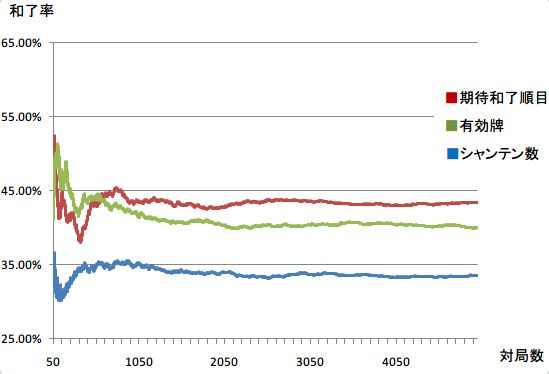
\includegraphics[keepaspectratio, scale=0.8,bb=0 0 549 374]
      {img/1houra.jpg}
 \caption{1人麻雀の和了率遷移}
 \label{1houra}
\end{figure}

\begin{table}[h]
  \caption{100局のデータセットでの和了率}
  \label{100houra}
  \begin{center}
  \begin{tabular}{c|c}
    \hline
    手法   & あがった局数(\%)\\\hline\hline
    上級者 	& 53 \\\hline
    期待和了巡目 & 44 \\\hline
    有効牌 	& 41 \\\hline
    平均プレイヤ 	& 36\\\hline
    シャンテン数	& 32 \\\hline
  \end{tabular}\end{center}
\end{table}

1人麻雀を5000局打たせたことによる和了率の比較では、「シャンテン数」<「有効牌」<「期待和了巡目」という結果となった。これは統計的に優位な水準での優劣である。結果については期待通りで、シャンテン数を下げるだけのアルゴリズムに対し、それをさらに有効牌の数を比べるアルゴリズムでは和了率が上昇した。また、本研究で提案した「期待和了巡目」のアルゴリズムでは、さらに有効牌の中でもより和了までの到達度を正確に計算することで和了率が上がることが確認された。1人麻雀による対局では、多人数性が存在しないため、本手法がうまく適用できると考えられる。また、上級者と平均実力者の人間プレイヤーを加えた100局の対局では、期待和了巡目のアルゴリズムの和了率は平均プレイヤーより優り、上級者に劣る結果となった。これは、上級者の場合はシャンテン数が瞬間的にあえて最小でないような打牌をして結果的に和了率がもっとも高くなる場合が存在するからであると考えられる。期待和了巡目はシャンテン数が最小になる牌の中から打牌を選択しているため、このような選択が行えない。
% \subsection{期待平均和了順目の探索の深さの評価}
% \subsection{モンテカルロ法の探索領域}


\section{4人麻雀における成績の評価} %麻雀サーバーとの対戦
本研究では1人麻雀における和了率の上昇を目指すため、静的指数である期待和了巡目を利用し、打牌を決定するアルゴリズムを提案した。これを第4章で設計した実装を元に、オンライン麻雀天鳳で打たせ、その成績を集計した。対戦した場所は天鳳の一般卓で、ルールは喰いアリ赤アリの東風戦、持ち時間は3秒である。2016年11月から2017年1月までの期間対戦を行い、試合数は2231戦となった。同じように、関連研究では1人麻雀のアルゴリズムを4人麻雀に適用し、実際の対人戦でその成績を評価している例が存在する。この節では、それらの研究の成績と本手法の比較を行い、その優位性を評価した。

評価として、和了率、放銃率、レーティングを比較した。


\subsection{和了率}
4人麻雀で実装した自動打ちシステムを対戦させた結果の、和了率の遷移を図\ref{houra2231}に示す。
50戦以下の対局では母数が少ないために和了率の偏差が大きいため、図は50戦以上の対局からの和了率を掲載した。和了率は300戦までは偏差が大きかったが、500戦を超えると徐々に収束していき、2231戦後の最終和了率は21.290%となった。

\begin{figure}[h]
 \centering
 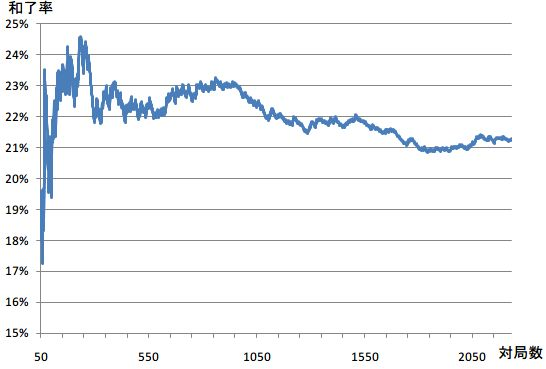
\includegraphics[keepaspectratio, scale=0.8,bb=0 0 546 369]
      {img/houra2231.jpg}
 \caption{和了率遷移}
 \label{houra2231}
\end{figure}

また、関連研究と比べた結果の表\ref{tb:houraritu}に示す。
佐藤らは有効牌を数え上げることによって打牌を選択するアルゴリズムを使用したが、その中で再帰の深さを変えたりヒューリスティックを加えたり複数の手法においてのデータを取っている。ただしそれらによる差は統計的に優位なほど大きな差ではなかったため、今回はそれらの中で最も基本的である再帰の深さ1のものと比較した。また、表にある平均プレイヤーとは、天鳳において平均レートが1500付近である初段のプレイヤーとした。そのデータは天鳳のランキングページに公開されているものを引用した。

\begin{table}[h]
  \caption{4人麻雀においての和了率の比較}
  \label{tb:houraritu}
  \begin{center}
  \begin{tabular}{c|c|c|c|c}
    \hline
    プレイヤー   & 本研究 & 佐藤らの研究 & 水上らの研究 & 平均プレイヤー\\\hline\hline
    対局数   & 2231 & 2526 & 504 & -\\\hline
    和了率(\%) & 21.3 & 20.1 & 18.8 & 21.9\\\hline
  \end{tabular}\end{center}
\end{table}

和了率を比較すると、本手法は佐藤らの研究をわずかに上回る結果となった。佐藤らの研究では有効牌の数え上げによって打牌を選択しているが、本手法では平均和了巡目を用いることでより先の展開を考慮した打牌の選択が可能になっていると考えられる。これは事前に期待されていたとおりであった。しかし、大きな差が生まれたというわけではなく、平均プレイヤーを優位に超えることはできなかった。これは、平均プレイヤーは鳴きによる和了も含まれているためであると考えられる。その理由に、1人麻雀による和了率(鳴きを含まない)は平均プレイヤーを超えていることがあげられる。ただし、4人麻雀でこれ以上の和了率を挙げるためには、やはり鳴きについての和了を加えないと難しいこともわかる。


\subsection{放銃率}
次に、和了率の遷移を図\ref{houra2231}に示す。
50戦以下の対局では母数が少ないために放銃率の偏差が大きいため、図は50戦以上の対局からの宝珠率を掲載した。放銃率は500戦までは下降を続けたが、1000戦を超えると徐々に収束していき、2231戦後の最終放銃率は18.377%となった。
\begin{figure}[h]
 \centering
 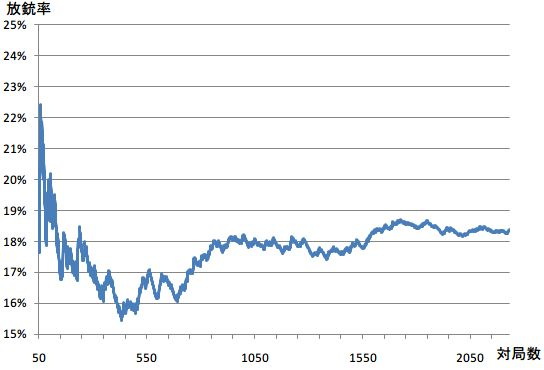
\includegraphics[keepaspectratio, scale=0.8,bb=0 0 544 370]
      {img/houzyu2231.jpg}
 \caption{放銃率遷移}
 \label{houzyu2231}
\end{figure}

また、関連研究と比べた結果を表\ref{tb:houzyu2231}に示す。
放銃率においてはどの研究にも大きな差は見られなかった。これらの研究では、4人麻雀におけるオリの戦略を加えていないからであると考えられる。平均プレイヤーはオリを行っているため、放銃率が低い。4人麻雀においては放銃率による失点は成績を悪くするため、重要な指標であるが、これらはオリの戦略を実装することで改善する必要があると考えられる。

\begin{table}[h]
  \caption{4人麻雀においての放銃率の比較}
  \label{tb:houzyu2231}
  \begin{center}
  \begin{tabular}{c|c|c|c|c}
    \hline
    プレイヤー   & 本研究 & 佐藤らの研究 & 水上らの研究 & 平均プレイヤー\\\hline\hline
    対局数   & 2231 & 2526 & 504 & - \\\hline
    放銃率(\%) & 18.4 & 18.9 & 19.0 & 16.4\\\hline
  \end{tabular}\end{center}
\end{table}

\subsection{レーティング}
レーティングとは、特定のプレイヤーが他のプレイヤーと比較してどの程度成績が良いかを図る評価の仕方の一つである。
レーティングは、平均順位と負の相関を持ち、式\ref{rate}で計算される。ゲームを行ったときの卓の平均のレーティングを$R_ave$とし、ゲームの結果の順位を$Rank$、ゲームを行う前のレーティングを$R$とした時、そのゲームによって更新されるレーティングがR'である。初期の時点でのレーティング($R$)は1500である。
\begin{equation}
\label{rate}
\Large R' = R + (50 - Rank × 20 + \displaystyle \frac{R_ave - R}{40} ) × 0.2
\end{equation}

4人麻雀で実装した自動打ちシステムを対戦させた結果の、レーティングの遷移を図\ref{rate2231}に示す。
50戦以下の対局では母数が少ないためにレーティングの偏差が大きいため、図は50戦以上の対局からのレーティングを掲載した。レーティングは500戦までは偏差が大きかったが、1000戦を超えると徐々に収束していき、2231戦後の最終放銃率は1382となった。

\begin{figure}[h]
 \centering
 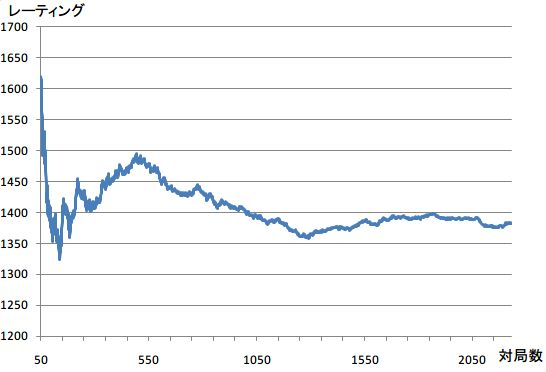
\includegraphics[keepaspectratio, scale=0.8,bb=0 0 546 372]
      {img/rate2231.jpg}
 \caption{レーティング遷移}
 \label{rate2231}
\end{figure}

また、関連研究と比べた結果を表\ref{tb:rate2231}に示す。
レーティングは佐藤らの研究をわずかに上回るという結果になった。しかし大きな有意差は見られず、平均プレイヤーにも及ばなかった。これは和了率の観点では本研究が優位なものの、四人麻雀では多人数性の理由によりほかの影響が多いことが考えられる。理由としては、1人麻雀では和了率が本研究の方が高いものの、放銃率では平均プレイヤーが低く出ているため、オリの影響が大きいと思われるからである。

\begin{table}[h]
  \caption{4人麻雀においてのレーティングの比較}
  \label{tb:rate2231}
  \begin{center}
  \begin{tabular}{c|c|c|c}
    \hline
    プレイヤー   & 本研究 & 佐藤らの研究 & 平均プレイヤー\\\hline\hline
    対局数   & 2231 & 2526 & - \\\hline
    レート & 1382 & 1339 & 1558\\\hline
  \end{tabular}\end{center}
\end{table}

% このように、レートは本手法の方が上回る結果となった。ここで保証安定レートについて比較をする。



